\chapter{Discussion}

This chapter presents a discussion around choosing an accelerometer for an ultra-low power application.

\section{Choosing An Accelerometer}

In almost any accelerometer based application, the accelerometer will do nothing 99\% of the time. From a power perspective, it is therefore most important to choose an accelerometer with a low sleep current. However, we still want the accelerometer to take measurements when movement is detected. It is therefore quite common for accelerometers to incorporate a low power wake-up mode. In this scheme the accelerometer use a very low measurement rate to listen for any motion above a certain threshold. When the threshold is breached, the sensors can enter normal operation and begin to sample at a much higher rate. From the comparison in Table \ref{tab:accel_comparison} we see that the ADXL362 from Analog Devices feature a motion detect mode which only consumes 270nA. In this mode the accelerometer samples at a rate of 6 Hz \cite{adxl362}, which should be more than enough to sense that an object is being moved. The threshold value can be specified in a dedicated register. When the specified threshold is breached, the accelerometer is able to respond autonomously by either entering full bandwidth measurement mode or by generating an interrupt. The ADXL362 also features an embedded FIFO that can hold 512 full resolution samples, which enables the accelerometer to autonomously collect samples without needing a poll request from the MCU. This is very beneficial, since it is often the MCU that consumes most power. The FIFO is also available in wake-up mode, which makes it possible to read out collected samples prior to the threshold breach. Some downsides with the ADXL362 is the relatively low output data rate, digital resolution of only 12-bits, as well as a relatively high spectral noise density. The last factor might be mitigated by using precision mode, but this comes at the cost of an increase in current consumption. The ODR rate and digital resolution might impose limitations on the number of applications that the accelerometer can be used for. The 6 Hz motion detect mode might noe be sufficient for detecting impacts. The LIS3DH and the KX123 both have a very high maximum ODR, and for these devices this mode is used to detect gestures such as double tapping. The closest competitor to the ADXL362 in terms of power consumtion is the MC3610 from mCube. This device uses 600nA in motion detect mode, which is over twice that of the ADXL362. One does however benefit from a better spectral noise density and a digital resolution of 14-bits. The MC3610 also have a FIFO, but it is only 32 samples deep. The LIS3DH from STMicroelectronics is also a interesting device. It has a high digital resolution of 16-bit, excellent spectral noise density and maximum ODR of 1.25kHz. It also has a lot of features, such as an embedded FIFO, free-fall and tap detection and a temperature sensor. Unfortunately the datasheet does not provide any numbers on current consumption for the wake-up mode. They do however state in an application note \cite{lis3dh_appnote} that the current consumption at 1 Hz ODR in low power mode is 2$\si{\micro\ampere}$. So it is very reasonable to assume that the current consumption will be somewhere in the $\si{\micro\ampere}$ range for this device. The MMA8491QR1 from Freescale Semiconductor has the lowest standby current and a digital resolution of 14-bit. A lot of the functionality in the device is automated, from power management to measurement range. This makes it simple for designer to use, but comes at a cost of reduced design flexibility. The device does not have FIFO, and only I2C is provided as digital interface. The supply voltage must also be greater than 1.95V for the device to work. 

The last device is the KX123 from Kionix. This features a very high resolution of 16-bit and a impressive 25.6kHz ODR. The KX123 also has a wake-up mode with a configurable measurement rate from 0.781Hz to 100Hz. At the lowest rate of 0.781Hz it consumes 1.8$\si{\micro\ampere}$. This is relatively much current when compared to the ADXL362 and MC3610. The supply voltage of 1.8V is also relatively high.

Based on this analysis, it is quite easy to point out the ADXL362 as the most power efficient accelerometer. With an overall best in-class wake-up and ODR current. It also has a large FIFO, which enables us to use the CPU less frequently and thereby saving power. 


\begin{center}
    \begin{tabular}{ | p{2cm} | p{5cm} | p{5cm} |}
    \hline
    Device & Pros & Cons \\ \hline
    ADXL362 & Lowest wake-up current \newline Lowest ODR current \newline Voltage operation at 1.6V \newline 512 Sample FIFO \newline SPI interface  & - \\ \hline
    \end{tabular}
\end{center}

\subsection{Are we sometimes able to completely turn off the accelerometer?}

As we see from table \ref{tab:accel_comparison} the lowest current consumption is in standby mode. A question arises from this, are we at some point able to assume that no motion is going to occur. If so, are we able to enter standby mode to further consume power? This scheme would require some external timer to wake the accelerometer. And one also need to assume that this timer is going to use less current than the wake-up mode itself. For most applications it would not be possible to predict whether motion is going to occur or not.

\section{Demo Board}

A demo board was created to show some potential IoT applications that can be achieved with ultra low power sensor data acquisition. 

The ADXL362 from Analog devices was chosen 

\subsection{nRF51}

The nRF51 is a Cortex-M0+ based System-on-Chip (SoC) from Nordic Semiconductor. The company is world leading in creating Bluetooth Low Energy solutions. This SoC was chosen mainly because of its advanced power saving features. 

The nRF51 features several serial interfaces. However, only the SPI module has DMA capabilities. It is therefore necessary to choose an accelerometer with an SPI interface. This only rules out the MMA8491QR1 from Freescale Semiconductor.

For optimal power efficiency it is optimal to use the lowest possible supply voltage. The nRF51822 can go as low as 1.8V.

\begin{center}
    \begin{tabular}{| l |}
    \hline
    6.3mA - TX at -4dBm (3V using on-chip DC-DC) \\ \hline
    8.0mA - TX at 0dBm (3V using on-chip DC-DC) \\ \hline
    11.8mA – TX at +4dBm (3V using on-chip DC-DC) \\ \hline
    9.7mA – RX (3V using on-chip DC-DC) \\ \hline
    13mA – RX at 1Mbps (No DC-DC) \\ \hline
    10.5mA – TX at 0dBm (No DC-DC) \\ \hline
    0.6µA – SYSTEM-OFF, no RAM retention \\ \hline
    1.2µA - SYSTEM-OFF, 8KB RAM retention \\ \hline
    2.6µA - SYSTEM-ON, All peripherals in idle mode \\ \hline
    \end{tabular}
\end{center}

\subsubsection{Programmable Peripheral Interconnect (PPI)}

The nRF51 features something the company calls Programmable Peripheral Interconnect (PPI). The PPI enables different peripherals in the device to interact autonomously with each other using tasks and events without using the CPU. The PPI can automatically trigger a task in one peripheral as a result of an event occurring in another. For instance, an interrupt from an external device (i.e. accelerometer) can trigger the SPI module to initiate a block transfer to memory. 

\subsubsection{EasyDMA}

The EasyDMA function in the nRF51 is able to move data to and from RAM and autonomously between peripherals. The DMA can be configured to work in conjunction with the PPI system for fully autonomous operation.

So in turn one should be able to make a sensor data acquisition system that is able to collect accelerometer data and send it over radio without using the CPU.

\subsubsection{Bluetooth Low Energy}

...maybe add something about Bluetooth Low Energy.

\section{The Configuration}

The planned example will utilize EasyDMA, PPI, SPI and the radio of the nRF51, as viewed with red boxes in Figure \ref{fig:accel_working_principle}. The Cortex-M0+ CPU should only be used for configuration of the system, and will be sleeping during data collection. The ADXL362 is configured to wake up when motion is detected, and then collect samples autonomously into its embedded FIFO. When the FIFO is full, the ADXL362 will send an interrupt to nRF51. The PPI is configured to listen to for this interrupt and to trigger a SPI block transfer when it is detected. As data is being transferred to the SPI module, the EasyDMA shuffles data either into the RAM or the radio module. This entire operation is possible without any CPU intervention.

\begin{figure}[h]
\centering
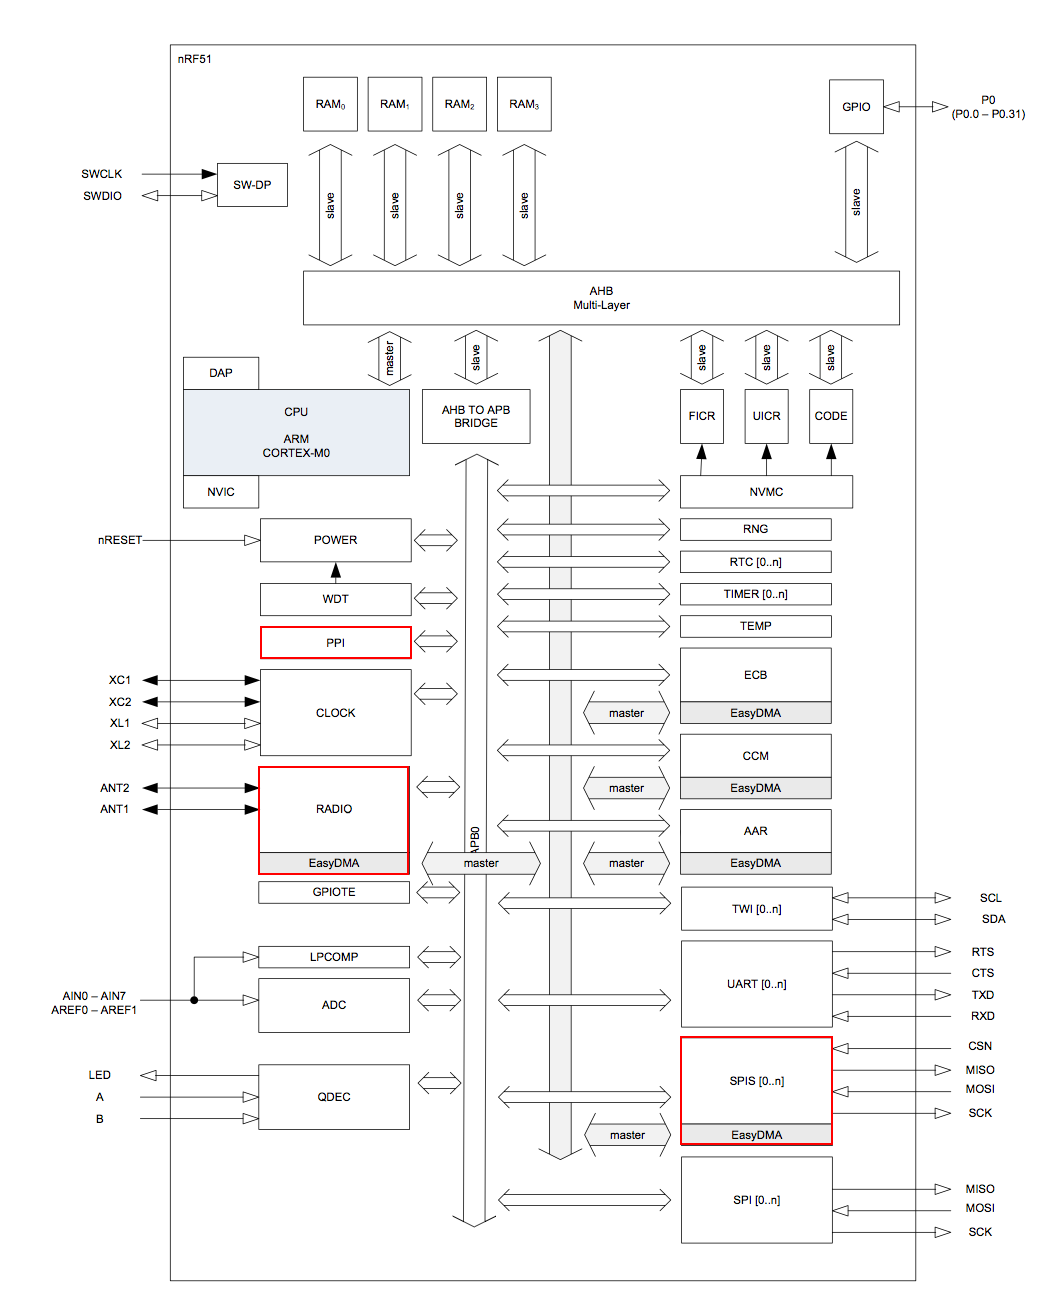
\includegraphics[scale=0.5]{fig/nrf51822_edit.png}
\caption{Nordic nRF51 System architecture. \cite{nRF51}}
\label{fig:accel_working_principle}
\end{figure}

\subsection{Power Estimation}

\begin{equation}
I_total = 1.2µA + 0.6µA
\end{equation}

\section{Possible IoT Application}

This section discusses some possible IoT applications for ultra-low power accelerometers. 

\subsection{Vibration Detection}

For some construction applications it can be very beneficial to be able to monitor the vibrations inside the structure itself. Ultra low power sensors can for instance be submersed inside concrete walls and transmit during the entire life-span of the building. From this application one can really see the problem with changing batteries. As one would literally need to tear down the wall to change batteries. 

\subsection{Motion Detection}

Motion Sensing is something that is being widely used in electronic devices today. It is for example being used as control input for certain smart phone applications.

\subsection{Health Monitoring}

Fitness armbands, smart watches and so on.

%%=========================================

\section{Background}
%In this section, you should present the problem that you are going to investigate or analyze; why this problem is of interest; what has, so far, been done to solve the problem, and which parts of the problem that remain.
%%=========================================
\subsection*{Problem Formulation}

Modern embedded system features a lot of power saving techniques. The problem of this thesis evolves around using all of these techniques to acquire data from a ultra low power MEMS accelerometer with the lowest possible power consumption. Then use the results to conduct a feasibility study of which IoT application the solution will be best suited for.

\subsection*{Literature Survey}
%You should here present the main books and articles that treat problems that are similar to what  you are studying. If you,  later in your thesis, describe the ``state of the art'' -- with a detailed literature survey, you may just give a very brief survey here (approx. a quarter of a page). If this is the only literature survey, you need to go into more details. An objective of the literature survey is to show the reader that you are familiar with the main literature within your field of research -- so that you do not ``reinvent the wheel.''

%%=========================================
\subsection*{What Remains to be Done?}
%After you have defined and delimited your problem -- and presented the relevant results found in the literature within this field, you should sum up which parts of the problem that remain to be solved.
%%=========================================
\section{Objectives}

%The main objectives of this Master's project are
%\begin{enumerate}
%\item This is the first objective
%\item This is the second objective
%\item This is the third objective
%\item More objectives
%\end{enumerate}

%All objectives shall be stated such that we, after having read the thesis, can see whether or not you have met the objective. ``To become familiar with \ldots'' is therefore not a suitable objective.

%%=========================================
\section{Limitations}
%In this section you describe the limitations of your study. These may be related to the study object (physical limitations, operational limitations), to the thoroughness of the analysis, and so on.
%%=========================================
\section{Approach}
%Here you should describe the (scientific) approach that you will use to solve the problem and meet your objectives. You should specify the approach for each objective.

%If there are any ethical problems related to your approach, these should be highlighted and discussed.
%%=========================================
\section{Structure of the Report}
%The rest of the report is structured as follows. Chapter 2 gives an introduction to \ldots

\begin{remark}
%Notice that chapter and section headings shall be written in lowercase, but that all main words should start with a capital letter.
\end{remark}